\paragraph{}
The IGES\cite{IGES1983} files introduced in Sec.~\ref{lr_sec:IGES} are used as the bridge between the engineering design and the numerical analysis in the proposed method.
As a standard file format in engineering design industry, it is supported by almost all design softwares all over the world.
Consequently, it offers a possibility to minimize the human effort spent on mesh generation.

\subsection{Parse geometry in IGES file}
\paragraph{}
The IGES file provides all information that describe the geometric input.
Abstract structure of the IGES file that describe the 2D geometry can be regarded as a simple curve-surface structure.
In other words, it defines the geometric input as certain number of surfaces with their boundaries in different colors, which represent different materials in engineering practice.
Each surface contains a list of curve indices which are corresponding to the curve information described in IGES file.

\paragraph{}
When the IGES file is feed into the programme, each line in the directory entry will be parsed entity by entity.
Parameter in directory entry describe the type and reference to other useful values for the entity.
An entity may refer to one or many entities in directory entry.
Detail of the specification of each entity is explained in \cite{Nasr2007} in detail.

%=====================================================================================================================%
\subsection{Output to mesh generator}
\label{qdt_section:iges_output}
\paragraph{}
The output file that the mesh generator read in will be a shorter summary of the geometric input.
Boundary representation will be kept as the data structure to describe the geometric input.
However, some fields apart from the curves or the surfaces will be added.
In the output file, the geometry will be organized in key points, polylines and surfaces.
The key points define the coordinates of all points and polylines are used to represent all curves including NURBS curves for simplification.
NURBS curves can be used directly by the mesh generator as well in \ref{qt_sc:nurbs} but it is found that the computational cost in the calculation of the distance between points to NURBS curves surpasses the merits of using it directly.
The exact geometry can be retained by projecting the nodes on the boundary back to the origin NURBS curves at the end of the algorithm.

\paragraph{}
Representing a straight line with polyline can be natural, first and the last points will be enough to achieve an exact representation.
However, that is not the case for curves whose curvature is not always zero.
Although adding more key points can increase the quality of polyline representation, computational cost in calculating the distance increases at the same time.
Yet, having only few key points may result in a bad polyline representation which leads to a poor mesh quality.
Elements may be twisted after the nodes on the boundary are projected to the origin curves.
As a consequence, a quantified indicator that is able to control the number and the position of the vertices on the polyline can be necessary.

%=====================================================================================================================%
\subsection{Discretization of the circular arc}
\paragraph{}
The chord ratio can be a good indicator for circular arc.
The arc length to chord length ratio $\frac{a}{L}$ illustrated in Fig.~\ref{qt_fig:iges_chord_ratio} can be expressed in angle $\alpha$ as:
    \begin{equation}
        \frac{a}{L} = \frac{
            \sqrt{2-2\cos\alpha}
        }{\alpha}
        = \frac{
            2\sin\frac{\alpha}{2}
        }{\alpha}
    \end{equation}
%
The maximum angle $\alpha$ satisfy arc length to chord length ratio $\frac{a}{L} > 1-\epsilon$ with $
    \sin\frac{\alpha}{2} = 1 - \frac{x^3}{6} + O(x^7)
$ can be derived as:
    \begin{equation}
        \alpha < \sqrt{24 \epsilon}
    \end{equation}

    \begin{figure}[h!]
        \centering
        \scalebox{1}{
            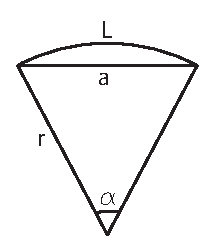
\includegraphics{quadtree/images/iges_chord_ratio.eps}
        }
        \caption{Chord length for circular arc}
        \label{qt_fig:iges_chord_ratio}
    \end{figure}
%
%=====================================================================================================================%
\subsection{Discretization of the NURBS curve}
\paragraph{}
For NURBS curves who have no closed form chord ratio, similar idea can be applied numerically.
The NURBS curve is first divided into serval smaller ones based on the knot vector as described in Sec.~\ref{lr_sec:nurbs_knot_ins}.  % may be explained in detail
Since the order of each subdivided NURBS curve used in engineering softwares are predominantly lower or equal to three, the sub-curves then can be divided into two classes, convex curves or concave curves with an inflection point as shown in Fig.~\ref{qt_fig:iges_chord_ratio_nurbs}.
    \begin{figure}
        \begin{subfigure}[b]{0.5\linewidth}
            \centering
            \scalebox{0.5}{
                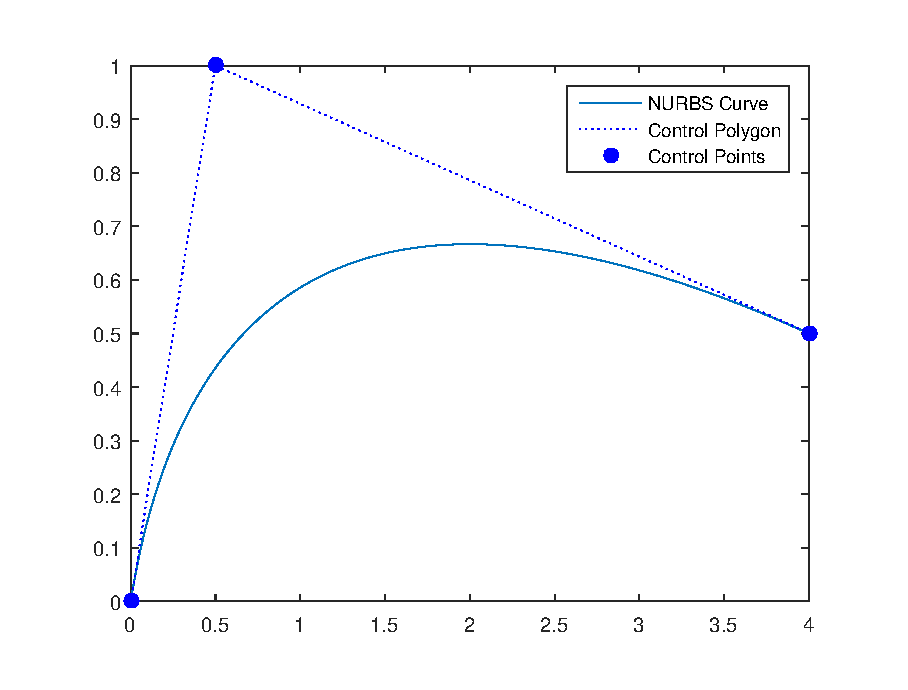
\includegraphics{quadtree/images/iges_chord_ratio_nurbs_convex.eps}
            }
            \caption{Convex}
        \end{subfigure}
        \begin{subfigure}[b]{0.5\linewidth}
            \centering
            \scalebox{0.5}{
                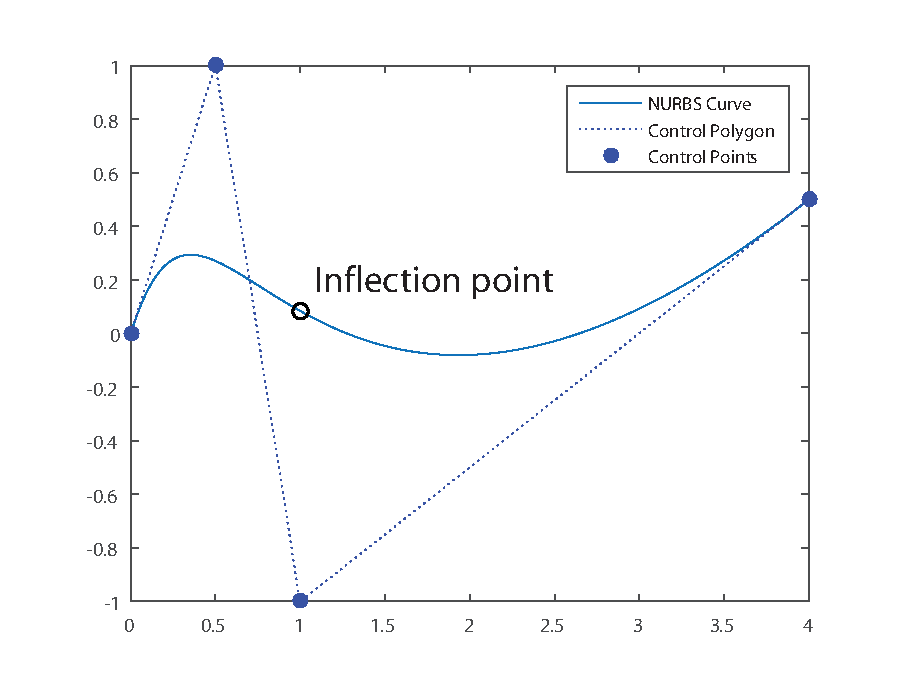
\includegraphics{quadtree/images/iges_chord_ratio_nurbs_concave.eps}
            }
            \caption{Concave with an inflection point}
        \end{subfigure}
    \caption{Type of sub-devided NURBS curves: convex and concave with an inflection point}
    \label{qt_fig:iges_chord_ratio_nurbs}
    \end{figure}
%
In order to determine the target NURBS curve is convex one or concave one, a cross product will be conducted.
by assuming the subdivided NURBS curve is cubic, there will be four control points $P_1,P_2,P_3$ and $P_4$.
If the signs of $cross(\overrightarrow{P_1P_2},\overrightarrow{P_2P_3})$ and $cross(\overrightarrow{P_1P_2},\overrightarrow{P_2P_3})$ are the same, then the curve is convex.
Otherwise it will be concave.

%=====================================================================================================================%
\subsubsection{Convex curves}
\label{qt_ssc:convex_curves}
\paragraph{}
Start with the simple case, in the situation illustrated in Fig.~\ref{qt_fig:iges_chord_split_convex_sum} where line $C(u_0)C(u_n)$ and the NURBS curve form a convex set, we are looking for a point $C(u_m)$ on the curve so that $C'(u_m)$ is parallel to $\overrightarrow{C(u_0)C(u_n)}$
    \begin{figure}[h!]
        \centering
        \scalebox{0.6}{
            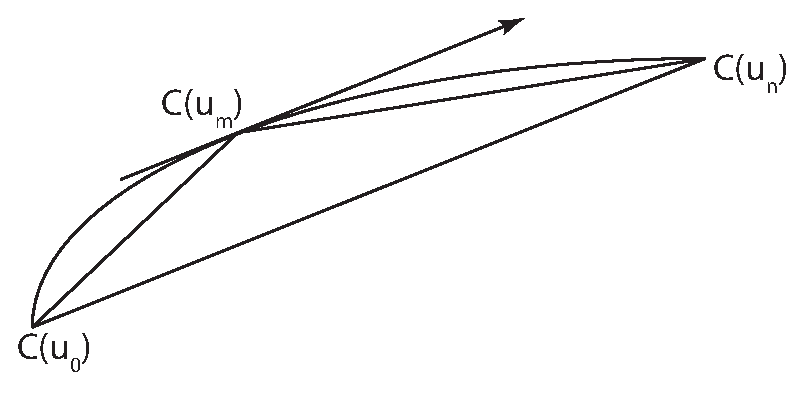
\includegraphics{quadtree/images/iges_chord_split_convex_sum.eps}
        }
        \caption{Discretization for convex NURBS curve}
        \label{qt_fig:iges_chord_split_convex_sum}
    \end{figure}
%
The target is to split one NURBS curve segment into two.
The splitting will be processed until the arc length to chord length ratio of any splitted curves are smaller than the tolerance.
Based on the property of the convex set, there can be one and only one parameter $u_m$ that satisfies the condition.
As a consequence, numerical methods such as Newton's method can be adopted to determine it.
For a given $u_m$, the next iteration will be:
    \begin{equation}
        u_{m_{new}} =  u_n - \frac{f(u_m)}{f'(u_m)}
    \end{equation}
%
where 
    \begin{equation}
        f(u) = C'(u) \begin{bmatrix}
            - C_y(u_n) + C_y(u_0) \\
            C_x(u_n) - C_x(u_0)
        \end{bmatrix}
    \end{equation}
%
The procedure to find $u_m$ can be concluded in Algorithm.~\ref{qdt_alg:split_convex_nurbs} and Algorithm.~\ref{qdt_alg:discrete_convex_nurbs} describes the procedure to find all knots corresponding to the vertexes of the polylines recursively.
\begin{algorithm}
    function splitConvexCurve(curve,u\_0, u\_n) \\
    \Input{
        curve, the input NURBS curve \\
        u\_0,u\_n, two end knots of the NURBS curve
    }
    \Output{
        u\_m, in Fig.~\ref{qt_fig:iges_chord_split_convex_sum}
    }
    u\_m = (u\_n + u\_0) * 0.5 \\
    pt\_0, pt\_n = getCurvePts(u\_0, u\_n) \\
    vector\_0n = Vector(pt\_0,pt\_n) \\
    angle = vector\_0n.atan2() \\
    deri1\_m = getCurveDeri(u\_m,1) \\
    angle\_m = deri1\_m.atan2() \\
    \While{abs(angle\_m-anlge)$<10^{-4}$}
      {
        deri1\_m, deri2\_m = getCurveDeri(u\_m,2) \\
        angle\_m = atan2(deri1\_m.y, deri1\_m.x)  \\
        fu = deri1\_m * vector\_0n.normalVector() \\
        fu\_deri = deri2\_m * vector\_0n.normalVector() \\
        u\_m = u\_m - fu / fu\_deri \\
        deri1\_m = getCurveDeri(u\_m,1) \\
        angle\_m = deri1\_m.atan2()
      }
    \caption{Split a convex NURBS curve into two}
    \label{qdt_alg:split_convex_nurbs}
\end{algorithm}
%
%
\begin{algorithm}
    function discreteConvexCurve(curve,eps,u\_0,u\_n,u)
    \Input{
        curve, the input NURBS curve \\
        eps, the tolerance of the chord to arc-length ratio \\
        u\_0,u\_n, two end knots of the NURBS curve
    }
    \Output{
        u, the vector of the knot corresponding to vertexes of the polylines
    }
    arcLength = curve.arcLength(u\_0,u\_n) \\
    chordLength = curve.getPt(u\_0).distanceTo(curve.getPt(u\_n)) \\
    \eIf{1-chordLength/arcLength $<$ eps}{
        return
    }{
        u\_m = (splitConvexCurve(curve,u\_0,u\_n))
        u.add(u\_m)
        discreteConvexCurve(curve,eps,u\_0,u\_m)
        discreteConvexCurve(curve,eps,u\_m,u\_n)
        return
    }    
\caption{Discrete a convex NURBS curve recursively}
\label{qdt_alg:discrete_convex_nurbs}
\end{algorithm}
%=====================================================================================================================%
\subsubsection{Concave curves}
\paragraph{}
As can be seen in Fig.~\ref{qt_fig:iges_chord_ratio_nurbs}, the extracted cubic NURBS curve will have no more than one inflection point.
The reason for that is because the target function is cubic and hence its second derivative will be in first order.
Consequently, numerical methods such as Newton's method can be used to find this unique point.
After that, the curve can be divided into two convex ones and the algorithms introduced in \ref{qt_ssc:convex_curves} can be used separately.
The Newton's iteration can be written as
    \begin{equation}
        u_{n_{new}} = u_n - \frac{f(u_n)}{f'(u_n)}
    \end{equation}

where
    \begin{equation}
        f(u) = C''(u)
    \end{equation}
%
%=====================================================================================================================%
\subsubsection{Calculation of the arc length}
\paragraph{}
The arc length of the NURBS curve defined on $u \in [u_0, u_n]$ can be expressed as
    \begin{equation}
        L = \int_{u_0} ^{u_n} \sqrt{C_x^2(u) + C_y^2(u)} du
    \end{equation}
%
The integration can be solved by the help of the numerical integration quadrature described in \ref{iso_subsection:numerical_integration} as:
    \begin{equation}
        L = \sum_{i=0}^n a_i \sqrt{C_x^2(u_i) + C_y^2(u_i)}
    \end{equation}
